\documentclass{beamer}

\usepackage{textpos}
\usepackage{amsmath}
\usepackage{amsfonts}
\usepackage{tikz}

% Commands
%For bold vectors
\newcommand{\uvect}[1]{\ensuremath{\mathbf{\hat{#1}}}} 	
\newcommand{\vect}[1]{\ensuremath{\mathbf{#1}}}
\newcommand{\del}{\ensuremath{\mathbf{\nabla}}}
\newcommand{\der}[2]{\ensuremath{\frac{\text{d} #1}{\text{d} #2}}}
\newcommand{\partder}[2]{\ensuremath{\frac{\partial #1}{\partial #2}}}


% Path to anjo-beamer/anjo
\newcommand{\anjopath}{/Users/andreas/beamer/anjo-beamer/themes/}
% Set anjotheme
\newcommand{\anjotheme}{Huskvarna}
% Set anjocolor
\newcommand{\anjocolor}{otter}

% Use packages
\usepackage{\anjopath beamertheme\anjotheme}
\usepackage{\anjopath beamercolortheme\anjocolor}

% Two logos
%\titlegraphic{\includegraphics[width = 0.1\textwidth]{irfLogo.eps}
%\vspace{0.3cm}
%\includegraphics[height = 0.1\textwidth]{uuLogo.pdf}}

% Title Information
\title{Really Important Science\\ In Space}

\author{Namn Namnsson$^{1}$\\
Some Name$^{1}$, Some O. Name$^{2}$ 
}
\institute[Universities Here and There] % (optional)
{
\inst{1}%
Institute of Space Lasers, University A

\inst{2}
Institute of Dinosaurs in Space, University B
}

\date{Important Conference, Uppsala\\ April 35, 2015}


% -- Adds a logo to every slide after the title --
% \addtobeamertemplate{frametitle}{}{%
% \begin{textblock*}{100mm}(0.1\textwidth,-1.3cm)
% \raggedleft\includegraphics[width = 0.1\textwidth]{irfLogo.eps}
% \end{textblock*}}


\begin{document}

%% ----Title frame------------
\begin{frame}
\titlepage
\end{frame}


%% ---------Second frame---------------
\begin{frame}
\frametitle{Second Frame}
\begin{itemize}
\item Lorem ipsum dolor sit amet, consectetur adipiscing elit. Sed quis ex malesuada, dapibus nunc at, condimentum sapien. 
\item Suspendisse rhoncus fringilla tellus sit amet fermentum. Nam mauris sapien, tempus gravida convallis sit amet, dapibus ac nisl.
\item  Sed efficitur eros eget dui fermentum, vitae suscipit nibh tincidunt. Suspendisse nisl metus, tempor at.
\end{itemize}

\end{frame}

% --------Thrid Frame----------------
\begin{frame}
\frametitle{Third Frame}
\begin{columns}
\begin{column}{.5\linewidth}

\begin{itemize}
\item Lorem ipsum dolor sit amet, consectetur adipiscing elit. Sed quis ex malesuada, dapibus nunc at, condimentum sapien. 
\item $\del \times \vect{B} = \mu_0 \left( \vect{j} + \epsilon_0 \partder{\vect{E}}{t} \right)$
\item  Sed efficitur eros eget dui fermentum, vitae suscipit nibh tincidunt. Suspendisse nisl metus, tempor at.
\item  Sed efficitur eros eget dui fermentum, vitae suscipit nibh tincidunt. Suspendisse nisl metus, tempor at.
\end{itemize}

\end{column}

\begin{column}{.5\linewidth}

\begin{figure}
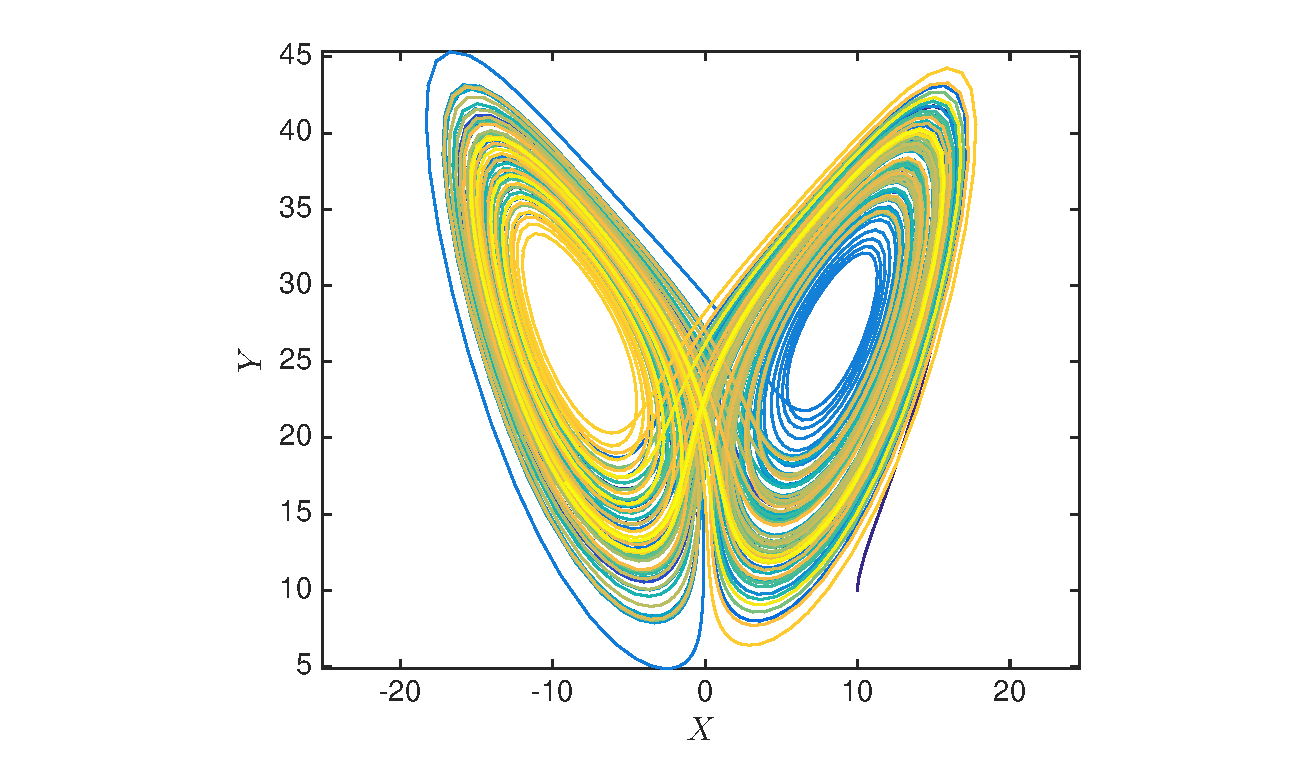
\includegraphics[width=\textwidth]{butterfly.eps}
\caption{Lorem ipsum dolor sit amet, consectetur adipiscing elit. Sed quis ex malesuada, dapibus nunc at, condimentum sapien. }
\end{figure}

\end{column}
\end{columns}

\end{frame}

% --------Fourth Frame----------------
\begin{frame}
\frametitle{Fourth Frame}
\begin{figure}
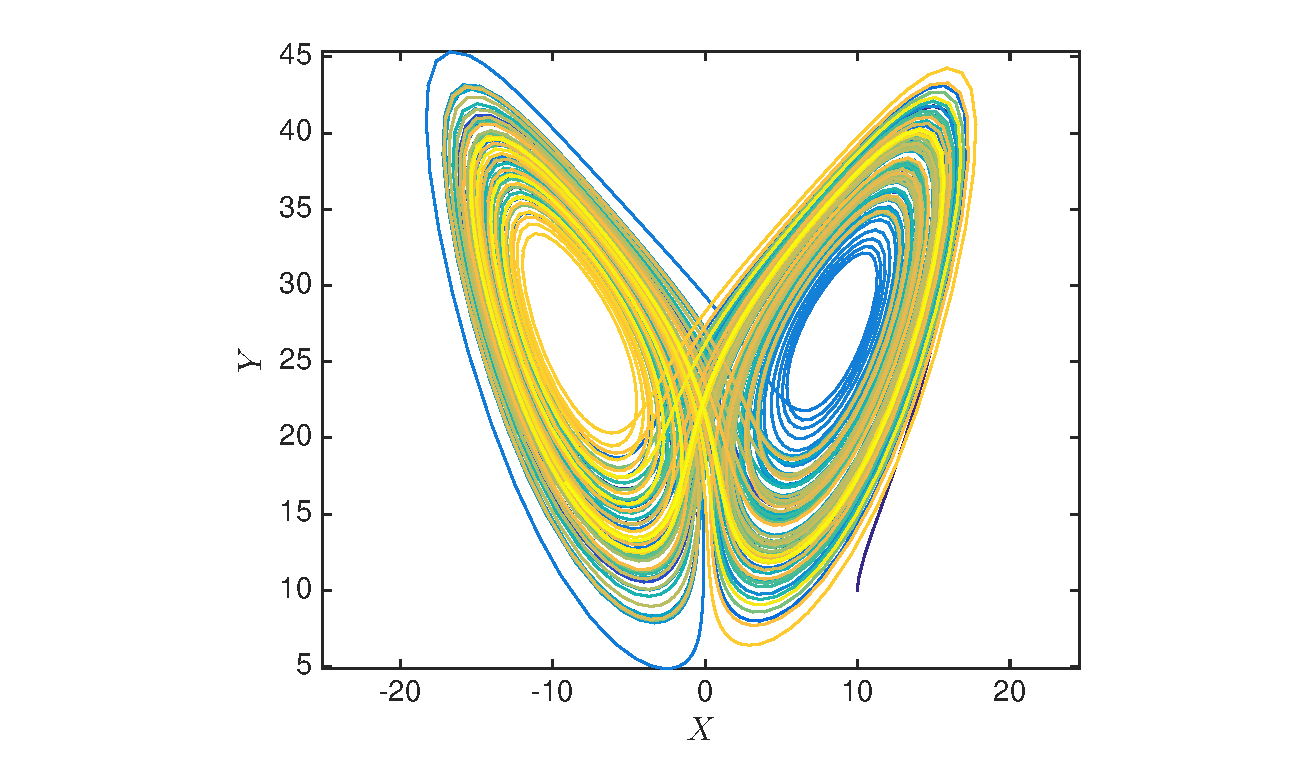
\includegraphics[width=\textwidth]{butterfly.eps}
\caption{Lorem ipsum dolor sit amet, consectetur adipiscing elit. Sed quis ex malesuada, dapibus nunc at, condimentum sapien. }
\end{figure}

\end{frame}

% --------Fifth Frame----------------
\begin{frame}
% Picture covers entire frame
% If picture is not wide, try [width=\paperwidth]
\begin{tikzpicture}[remember picture,overlay]
\node[at=(current page.center)] {
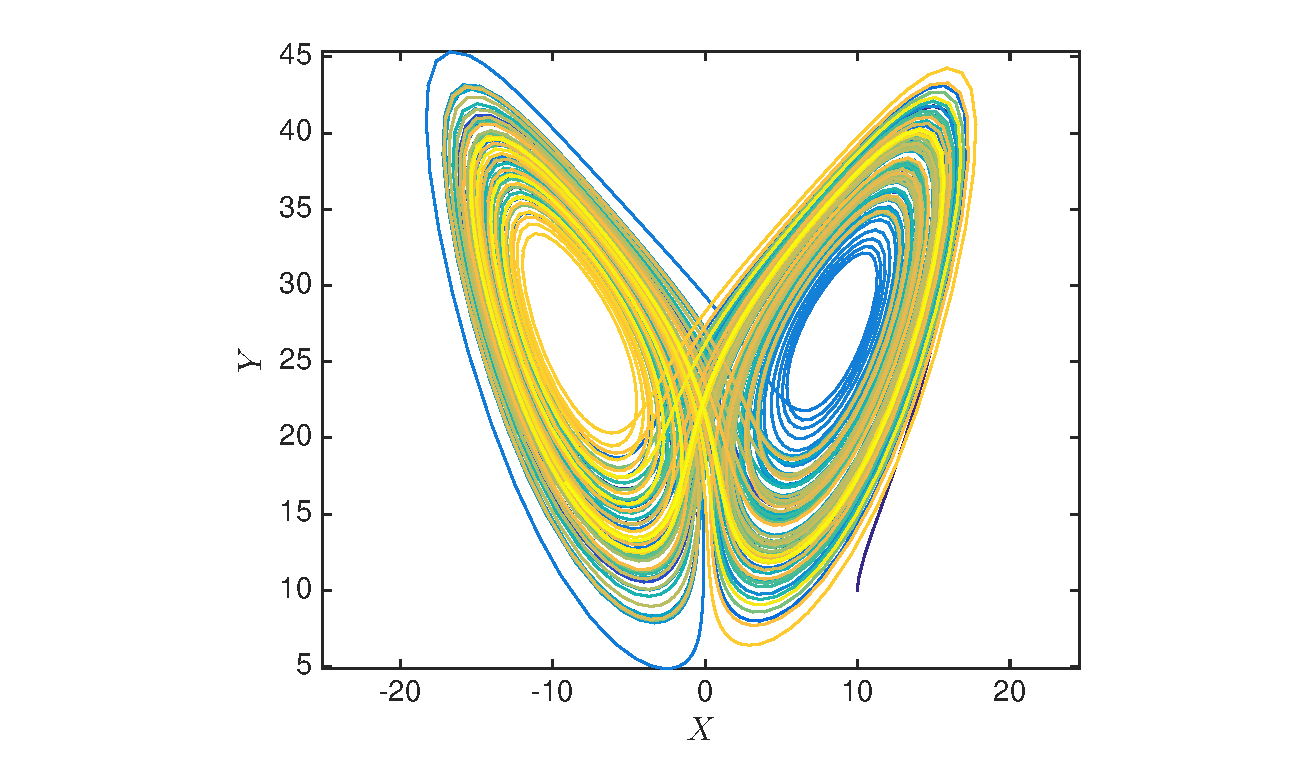
\includegraphics[height=\paperheight]{butterfly.eps}
};
\end{tikzpicture}
\end{frame}

% --------Reference Frame----------------
\begin{frame}
\frametitle{References}   

\begin{thebibliography}{}
\bibitem[Caprioli et al.(2015)]{cap15} Caprioli, D., Pop, A.-R., \& Spitkovsky, A.\ 2015, ApJL, 798, L28

\bibitem[Carlisle(1995)]{1995C} Carlisle, D.~B.\ 1995, 
Dinosaurs, Diamonds, and Things from Outer Space, The Great Extinction, 
ISBN 0804723923, Cambridge University Press, Hardback, 1995.,  
\end{thebibliography}

\end{frame}

\end{document}